\documentclass[a4paper, 12pt]{article}
%\usepackage[a4paper,hmargin=3cm,vmargin=3cm]{geometry}
\usepackage[english]{babel}
\usepackage[applemac]{inputenc}
\usepackage[sc]{mathpazo}
\linespread{1.05}         % Palatino needs more leading (space between lines)
\usepackage[T1]{fontenc}

\usepackage{amsmath}
\usepackage{hyperref}
\usepackage{graphicx}

\newcommand{\link}[1]{\href{http://#1}{\texttt{#1}}}

\newcommand{\code}[1]{\texttt{#1}}

\title{Reinventing 2048 \\ \large{An ITSMAP Project Report}}
\author{Kristoffer Andersen \\ \large{20103316} \and
Christian Clausen \\ \large{20081015}}
\date{$6^{th}$ of June, 2014}

\begin{document}
% Front page
\pagenumbering{gobble}
\maketitle
\newpage
% TOC
\tableofcontents
\newpage
\pagenumbering{arabic}

\section{Introduction}
The game known as 2048 went viral in 2014 when Gabrielle Cirulli
posted a simple game with a 4 by 4 grid with the squares from 2 to
2048 on Github. The game play was self-explanatory, the visuals
timeless and a viral hit was born.

Since then the game has spawned numerous variations, but for a game
with such obviously touch-friendly input, the variations in the mobile
market has been few and far between.

This report presents a reimplementation of Cirulli's 2048 from scratch
in the native Android Framework, but with a twist: we wholly embrace
the prospects that the app is running on a mobile device.

We proceed with detailing a specification of the problem, and
explicating in what ways our vision is different from the original. We
then go on to sketch some of the architectural decisions that we made
in order to facilitate our design. Finally, we detail the Android
Framework features that we made use of, in addition to the features
that we \emph{could} have made use of. Additionally, we bring a work
plan in the appendix, detailing who did what on the project.

\section{Specification}
% Requirements specification (Comments and sketches like GUI)
The goal with our app is to provide the basic 2048 experience. As
such, we here briefly outline the classic game mechanics, for the
readers that are not familiar with it.

\subsection{Core Game Mechanics}

The game is played on a quadratic grid with four squares to a
side. During the course of the game, the grid is filled with tiles
that can be slid across the grid. The only four actions the player can
take is to slide all tiles across the grid in one of the cardinal
directions: up, down, left and right. \emph{Playing} the game thus
amounts to deciding a sequence of these directions.

The tiles are numbered with subsequent powers of 2, starting with
2. When two tiles with the same value collide, they merge to a new
tile with the sum of the two involved numbers. That is, as tile with
the number 32 collides with another tile with the number 32, they
merge to form a new tile with the number 64.

The objective of the original game is to form a tile with the number
2048. When two tiles merge, the player is also awarded the sum of the
two tiles in points.

When the player has made a decision, resulting in a changed board, the
game places a new tile in a randomly chosen empty cell, with the value
2 or 4.

The dynamics of the game thus arise as the board fills up, making it
more difficult for the player to merge tiles. And, as the game
progresses, the average value of the tiles already on the board
increases, and as such it becomes more difficult to use the new 2 and
4 tiles the game places.

The game is over when there are no more moves that would result in a
tile moving or two tiles merging.

\subsection{Variations}

The game as described in the previous section is how Cirulli published
it in 2014, with a 4 by 4 grid and the tiles from 2 to 2048. It was
implemented in JavaScript, and used the arrow keys as input. Simple
\emph{WebView}-style apps were made for the Android and iOS platforms
with touch based input, where a swipe in the cardinal directions
results in the corresponding move in the game.

However, the fact that Cirulli decided to publicly release the
intellectual properties associated with the game, the fact that the
game is hosted on GitHub (such that with one click, one gets a
complete, hosted copy of Cirulli's game to alter as one sees fit, live
and on the Internet from the very first moment), combined with its
accessibility, and addictiveness has meant that it has inspired
countless variations.

Some variations extend the dimensionality of the grid on which the
game is played. If the game as envisioned by Cirulli is played on a
plane, the 3D version is played \emph{in} a cube, and so on. We lack
prepositions in the English language to describe how games are played
in four dimensions and beyond, but the variations exist, readily up to
at least 6 dimensions. To be able to fathom and play such a game is
one thing; from a technical stand-point, it is interesting to consider
how to control such a game. While the arrow keys, or a swipe on a
touch screen are completely believable analogies to movement in two
dimensions, it becomes much more difficult to come up with controls by
analogy once the game extends three dimensions. Most implementations
simply give the player yet another pair of keys to control movement
along the given dimensions. We will return to this point shortly.

Other variations play on the esthetics of the app, with pictures,
popular internet memes, operators from the creator's favorite
programming language, and so on. While entertaining and clearly a
contributing part of the game as a phenomenon, it is from a technical
perspective not very interesting.

Some variations are outside of a general description. A favorite
implementation of ours is a democratized version: every player dials
in to the server and ``votes'' for what the next move will be, as
opposed to playing it directly. The social angle is definitely a
contributing factor to the success of the app, and this is playing
that to the extreme.

It would not surprise us if the number of variants is approaching
2048; there are far too many to cover them here. For a more complete
list we refer to \link{http://phenomist.wordpress.com/2048-variants/}.

\subsection{Vision}

We wish to investigate the input design-space. The idea originated
from brainstorming what would make it possible to exhibit the features
of the Android Framework and a mobile platform in a fun and obvious
way.

To make a general statement about the controls required for the game,
we drew inspiration from the higher dimensionality variations that
have been made, where they rather weakly just added another key-pair to
the set of controls. As such it becomes obvious that an input device
for a game 2048 must just be able to produce two discernible, discrete
signals in order to control movement along an axis. 

Our vision with this prototype is to build an app that allows the
prototyping of input control methods to a game of 2048. Mobile devices
offer such a wealth of sensory input that a classic desktop setting
simply cannot compete. 

\subsection{Specification}

The app has to...
\begin{itemize}
\item ... provide the basic functionality, look and feel of a game of 2048.
\item ... allow the user to select different input methods.
\item ... provide an on-line high score service, in order to make use
  of the connectivity features of the Android Platform and to enhance
  the social aspect of the game.
\item ... provide application developers with a framework for
  prototyping new input method variations for games of 2048.
\end{itemize}

\section{Software Architecture}

So there are two intrinsic forces guiding our hand in the design of
this app. For one, it is an important consideration that we are
working on the Android Platform. It has unavoidable consequences while
offering unique opportunities. Secondly, we wish to build as flexible
an app as possible, in order to facilitate easy extension of the
collection of possible user input methods.

The basic game logic is handled through a software architecture
classic: the Model View Control pattern. The pattern is a OO oldie,
and an architecture centered around the MVC pattern gives a range of
benefits. Primarily it solves two problems given one assumption: data
is shared. Problems then arise when we realize that the ways we wish
\emph{to manipulate} and \emph{to visualize} it is variable, perhaps
even undetermined. The MVC pattern then defines three \emph{roles}:
the model, the view and the controller. The model has the
responsibilities of maintaining the state of the data, and to notify
the data visualizers (the views) when the data changes. The views have
the responsibility of visualizing data, and possibly pass on the user
interactions with the views as events to the controllers, who bear the
responsibility of translating these events into state changes on the
model.

The overall architecture is illustrated with the concrete interfaces
of our app playing the roles of model, view and controller in the UML
diagram in Figure \ref{fig:mvc-1.png}.

\begin{figure}[!h]
  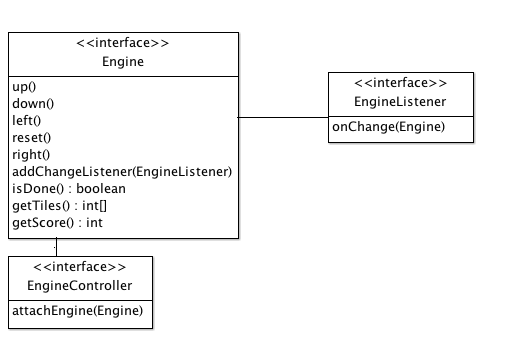
\includegraphics[width=\linewidth]{mvc-1.png}
  \caption{The MVC pattern as implemented in our 2048 app}
  \label{fig:mvc-1.png}
\end{figure}

The data that we store in our game is the state of the game board and
the user score. This state also gives rise to some derived queries
like the layout of the board (\code{getTiles()}) and whether the game
is over or not (\code{isDone}). This state is used to visualize the
state of the game, and whenever the game state changes the concrete
implementation of \code{Engine} is supposed to call \code{onChange} on
every registered EngineListener. These state changes are caused by the
concrete EngineControllers in play, who have access to the modifiers
of the Engine implementation. A minor twist on the classic MVC UML
diagram is that the controller \emph{also} exhibits an interface for
registering models, which we found necessary to handle the activity
life cycle with regards to resource handling in our app.

We have two concrete views in our game, as detailed in the full UML
diagram of the MVC implementation found in \label{fig:mvc-2.png}. One
is the grid and the other is the \code{ScoreView}, a GUI element for
showing the score of the game.

\begin{figure}[!h]
  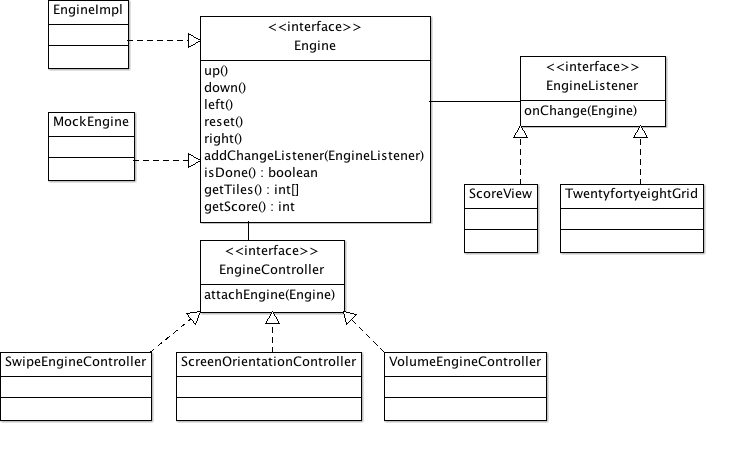
\includegraphics[width=\linewidth]{mvc-2.png}
  \caption{The MVC pattern as implemented in our 2048 app, with all
    concrete classes indicated.}
  \label{fig:mvc-2.png}
\end{figure}

The controllers shown each implement a way of interpreting user events
in terms of state updates on the game model. The volume key controller
intercepts key presses to the volume controls present on all Android
devices, and translates into either vertical or horizontal slides,
depending on which axis it was registered as controlling. The screen
orientation controller similarly controls an axis by using the
orientation around the horizontal axis as reference for motion
events\footnote{We have found it works best for controlling the
  horizontal axis!}. Finally, the swipe controller is a little
interesting as it plays a role in two frameworks. For one, it's a
controller in our MVC pattern. But then, it is also a \emph{listener}
in the Observer pattern used by the Android Framework in order to
handle events. As such it must be registered with a View (note, of the
Android Framework GUI variety, not our pattern!) in order to receive
input events. The \code{TwentyfortyeightGrid} plays a similar dual
role, and so is aptly suited to act as the \emph{observed} object
needed in the Android Observer pattern. An entire exchange between the
\code{SwipeController}, the \code{TwentyfortyeightGrid} and the
\code{EngineImpl} is detailed in the sequence diagram in Figure
\ref{fig:seq-1.png}:

\begin{figure}[!h]
  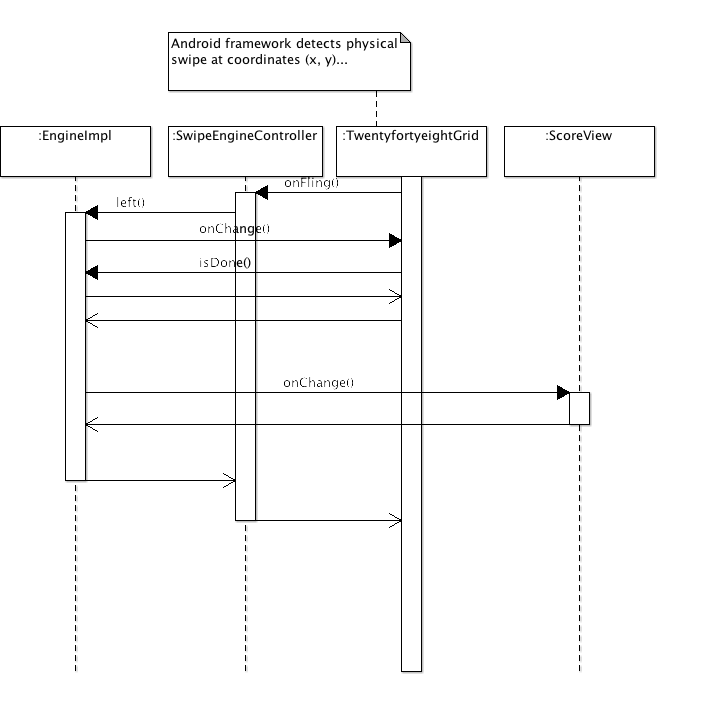
\includegraphics[width=\linewidth]{seq-1.png}
  \caption{A sample interaction between model, view and controller in
    our app.}
  \label{fig:seq-1.png}
\end{figure}

An unintended benefit gained from a strict implementation of the MVC
is the clean separation of concerns. The data is cleanly encapsulated
by the \code{Engine} interface. This means that testing with the
technique known as mocking is a breeze. We implement a simplified to
the point of triviality version of the game logic, such that it is
both deterministic and entirely predictable. This version can be found
in \code{MockEngine.java}, and was used while testing the various
controllers and views. This way, the random logic of the engine and
general complexity of the real engine minimally camouflaged bugs and
other errors in those components under the test. It's not quite unit
testing, but the technique did allow us to isolate the components
under the test under the assumption that the other components were so
simply mocked that they could not be wrong!

\section{Uses of the Android Framework}

We have used numerous parts of the Android Framework, each detailed in
its own subsection.

% We have used
% - Activities + Fragments + Intents
\subsection{Activities, Intents and Fragments}
One cannot create an Android app without touching these two parts of
the API. The activity and fragment abstraction clearly isolate ``doing
one thing'' on a mobile device, and intents allow for the transitions
between them. Logically, we have an activity and/or fragment for each
interaction a user can have with our app.

We have an activity displaying the main grid, for interaction with the
game state and the submission of high-scores. We have an activity for
the display of submitted high-scores. We have a fragment for changing
the active input method, and we have a fragment for displaying
licensing details where we pay homage to the original 2048 in addition
to the people making the font we used available.

The use of fragments is key to making dynamic layouts. Unlike its
competitor, the iOS platform, an Android app should expect to run on a
countless number of hardware configurations, with varying screen
sizes, resolutions and aspects to say the least. To that end, the
Android Framework provides isolated GUI and logic components known as
fragments, such that we can dynamically piece together one activity at
runtime, when the hardware the app is running on is known.

We exploit that in our app by displaying the possible settings in the
classic list of settings with a main view in the middle configuration
when on large screens and a list switching to a full screen settings
fragment on smaller screens, just as we practiced in the hand-ins for
the course. This allows us to utilize the screen maximally.

The main activity is locked in portrait mode in order to preserve the
feel of the original 2048, but something similar could be done with
the main screen, where, depending on orientation of the screen, the
button are to either side as opposed to just above the grid.

% - Preferences
\subsection{Preferences \& Permanent Storage}
The possibility of the user configuring our app is key to making it
work. Firstly, we require the persistence of configurations across
activity boundaries, such that we can navigate to our settings
activity and back to the main activity with altered input methods.

This could be done in-app with the message passing style that intents
facilitate. However, we would also like for the users preferences to
persist across sessions of interaction with the app, such that their
favorite input method remains selected, even once the app is closed.

This is precisely what the Android Framework offers through its
\emph{Shared Preference} API. The shared preferences are a simple,
key-value persistent storage of primitive types, which we use to store
the input methods the user has selected. Simple and effective.

We could have made use of more severe permanent storage like a SQLite
data store, but that would frankly be overkill for two integers.

% - Externalization
\subsection{Externalization}
We make use of externalization, in order to achieve flexible code, and
an adaptive app. Externalization embodies a classical computer science
saying: any problem can be solved by yet another layer of
indirection. By introducing a layer of indirection, the running code
becomes unaware of \emph{what concrete value} it is manipulating at
run time, only \emph{the name} it can refer to that value by on
compile time. This simple ``trick'', if you will, is used to many
effects on the Android platform. 

\subsubsection{Layouts}
By externalizing layouts into XML files, we can achieve dynamic
layouts. We used the trick taught through the obligatory course work:
by creating a reference to a larger layout that is only in effect on
large devices, we automagically use a more information-dense layout on
devices with large screens for out settings activity.

\subsubsection{Localization}
We have used Sequyoa as seen in the course, in order to dynamically
change the language between English and Danish. In this case the
Android Framework keeps track of the "strings.xml" file, and chooses
either the one located in "values" or "values-da" based on the user's
language settings.

\subsubsection{Colors}
The iconic style of the app is greatly defined by its colors, which
are consistent through out. We accomplish this by also externalizing
the colors into the "color.xml". This of course also means that we
could use different colors depending on the language, screen size, or
something like that, but we chose not to, as to preserve the look and
feel of the app.

% - Background tasking / Async
\subsection{Background Tasks}
In parts of the project we wish to display information, that is not
readily available, such as the license files, stored on the phone, or
the high-score stored on a server. In these cases it makes sense to
collect and prepare the information in a background task, so the user
isn't necessarily bothered by any possible wait there might be while
loading the data. The user should never feel like the app is
unresponsive. After loading the data we could have used broadcasts to
signal that an update to the view needs to occur, but since the view
has the background task, we chose the simpler option and let the task
update the view directly.

% - External services (RESTful servers) (+ Content Provider?)
\subsection{External Services}
In our app we wish to share information among all of our users, namely
the high-score list. Therefore we have to use some external service to
store the information on the internet.

We chose to have the high-score information stored on a RESTful server,
that can be accessed through the JSON format, which we have previously
worked with during the course. Thus we here follow the same structure:
Create a URL, then a GetRequest, convert the input stream to a string,
and then use Java's built-in libraries for JSON to parse the
string. This way we could easily extend the project to store other
informations such as the geolocation of each high-score, names, time of
day, language, screen size, and so on. We could even extend the server
with any of these, without changing anything in the Android code.

% - Managers needed for device sensors
\subsection{Device Sensors}
We could not have done this app without the input and sensory hardware
capabilities of a mobile platform like Android. As an example of a
hardware sensor we tapped from the software, we used the screen
orientation sensor, which is a software abstraction on top of the
hardware accelerometer built into the hardware. We used a software
listener to receive call-backs from the abstract sensor, and used these
events to play the role of a controller in our central MVC.

The screen orientation sensor is a simple sensor to work with,
particularly compared to something like the NFC, Bluetooth, WiFi or
GPS signals, the accelerometer and the ambient light sensor (when
that's present on the hardware!). All these have a more complicated
API which is why they weren't our first choice for integration into
the app, but on the other hand, we have established a perfectly good
MVC framework that can be easily extended with more controllers.

This area is the one we by far regret the most not having enough time
to explore further.

% - Toasts
\subsection{Toast}
A Toast is part of the Android framework, is a temporary pop-up
message. We use Toast messages to notify the user that his high-score
has been sent to the server, in order to provide a smooth, and
comfortable experience for the user. As previously mentioned the user
should never feel like the app is unresponsive, so when he presses a
button it helps to provide a visual response in the form of a Toast.

% - Custom views
\subsection{Custom Views}
Ah, our saving grace. The Android Framework provides several standard
GUI components and layouts known as views. These standard components
preserve the look and feel of the particular Android device, to give a
smooth and familiar experience for the user of your app, and a
pleasant development experience where one is spared reinventing the
wheel (or the button, in this case).

Some apps just call for a unique look and feel, like ours, and so the
framework provides the possibility for developer code to extend the
View class or any subclass like TextView, and overwrite the onDraw
method. OnDraw takes a Canvas object representing a brush with which
we can paint on the screen, and from then on the sky's the limit.

We used this facility extensively in the main screen to capture the
look and feel of Cirulli's 2048, in everything from an entirely new
kind of view in the grid to simply stylized buttons.

% We could have used
% - Network connections
% - Local storage?
% - Notifications

% Couldn't use?

\subsection{Content Provider}
A Content Provider functions as a local RESTful server, e.g. a local
SQL database in which you could store persistent data, provided you
get the permissions.

\subsection{The Java Language}
Finally, the Java programming language is a mature, well established,
well documented technology with which we are already familiar, having
been taught the language as part of our CS background. The ability to
code something as integral and admittedly a little delicate as an
MVC pattern ``as we usually would'', enabled speed and flexibility to
our development process.

Aspects like concurrency and collections libraries are where Java has
already made a name for itself, and the ability to leverage all that
on the Android platform is ingenious and invaluable.

On the other, this does mean you are coding in Java. Java is slightly
verbose and at times slightly cumbersome, lacking (more or less)
modern features like higher-order functions and algebraic data types. 

\section{Conclusion}
% Conclusion
What we have demonstrated with this project is how to develop a
functional and complete Android app. An app that uses Android features
such as touch, store preferences persistently, and communicates with a
RESTful server. We have succeeded in adapting a know design from a
web-service, into a mobile interface, and preserving the same
look-and-feel.

% Future Work
The project we have made, could be extended in a lot of ways, such as
the option of attaching ones name when you submit a high-score, or the
country one resides in, thereby we could add a second high-score list
by country, so users had another parameter to compete on, if they
didn't want to give up their name.

We could have also added animations, a different win screen, the
option of choosing a different sequence, or undo
functionality. Basically we could have incorporated almost any of the
variations, and with a flexible software design well established, the
extension along any of the three axes in the MVC pattern is easy and
reliable.

\newpage
\appendix
\section{Appendix: Work plan}
\subsection{Christian's Contribution}
\begin{itemize}
\item \code{src/dk/compsci/twentyfortyeight/}
  \begin{itemize}
  \item \code{HighScoreActivity.java}
  \item \code{EngineImpl.java}
  \end{itemize}
\item \code{res/layout/}
  \begin{itemize}
  \item \code{activity\_highscore.xml}
  \end{itemize}
\item The REST service running at \code{http://2048.compsci.dk/json.php}, and the use hereof.
\end{itemize}
\subsection{Kristoffer's Contribution}
\begin{itemize}
\item Everything not mentioned under \textbf{Christian's Contribution}
\end{itemize}

\end{document}